The sections below compares the experiments from section 3.1 to 3.4. 

\section{The AUC Performance of mixed Data Experiments}
I compared the AUC performance of source data model (B1), target data model (B2), and mixed data model (M1). The mixed data model highly improves AUC performance especially when the number of target data is small. It is a simple way to improve the performance by adding target data into training dataset. But the disadvantage is also clear. The calculation cost is huge since the number of training data is large compared with other methods.
 \\

\begin{figure}[H]
    \hfil
    \begin{minipage}[t]{0.9\textwidth}
        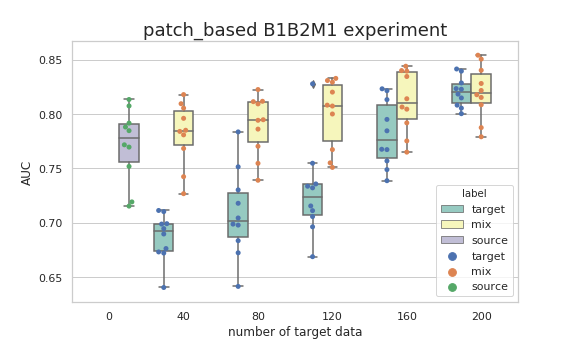
\includegraphics[width=\textwidth]{fig/B1B2M1_num_patch.png}
        \caption{\label{fig:parallel1}Patch-based AUC for B1B2M1 Experiment}
    \end{minipage}
    \hfil
\end{figure}
\begin{figure}[H]
    \hfil
    \begin{minipage}[t]{0.9\textwidth}
        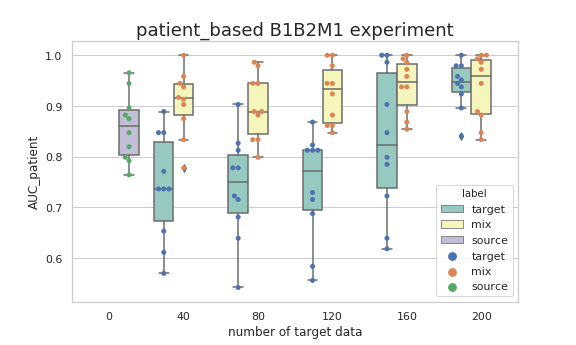
\includegraphics[width=\textwidth]{fig/B1B2M1_num_patient.png}
        \caption{\label{fig:parallel1}Patient-based AUC for B1B2M1 Experiment}
    \end{minipage}
    \hfil
\end{figure}

\section{The AUC Performance of Fine-Tuning Experiments}
I compared the AUC performance of source data model (B1), target data model (B2), and fine-tuning model (F1). The fine-tuning model highly improves AUC performance especially when the number of target data is small. It improves the disadvantage of mixed data model. The calculation speed is fast since it only need to train target data if we already have source data model. 
 \\

\begin{figure}[H]
    \hfil
    \begin{minipage}[t]{0.9\textwidth}
        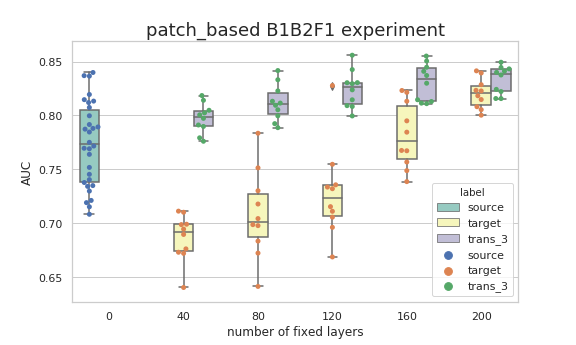
\includegraphics[width=\textwidth]{fig/B1B2F1_num_patch.png}
        \caption{\label{fig:parallel1}Patch-based AUC for B1B2F1 Experiment}
    \end{minipage}
    \hfil
\end{figure}
\begin{figure}[H]
    \hfil
    \begin{minipage}[t]{0.9\textwidth}
        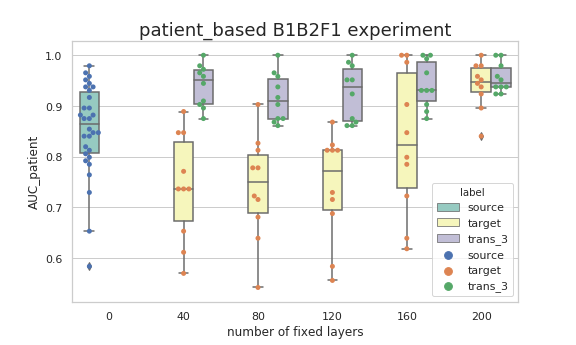
\includegraphics[width=\textwidth]{fig/B1B2F1_num_patient.png}
        \caption{\label{fig:parallel1}Patient-based AUC for B1B2F1 Experiment}
    \end{minipage}
    \hfil
\end{figure}


\section{Comparison of Mixed Data Experiments and Fine-Tuning Experiments}

I compared the AUC performance of source data model (B1), mixed data model (M1), and fine-tuning model (F1). mixed data model and fine-tuning model both improve the performance, but fine-tuning model performs better than mixed data model with lower calculation cost. Obviously fine-tuning method is a workable method to improve the AUC performance applied on target data. 
 \\

\begin{figure}[H]
    \hfil
    \begin{minipage}[t]{0.9\textwidth}
        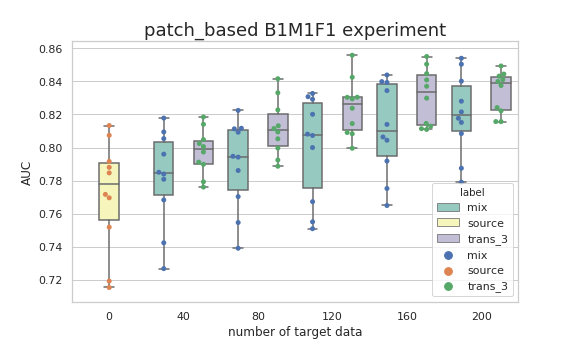
\includegraphics[width=\textwidth]{fig/B1M1F1_num_patch.png}
        \caption{\label{fig:parallel1} Patch-based AUC for B1M1F1 Experiment}
    \end{minipage}
    \hfil
\end{figure}
\begin{figure}[H]
    \hfil
    \begin{minipage}[t]{0.9\textwidth}
        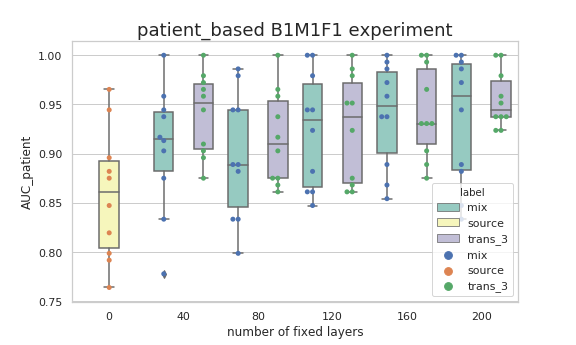
\includegraphics[width=\textwidth]{fig/B1M1F1_num_patient.png}
        \caption{\label{fig:parallel1} Patient-based AUC for B1M1F1 Experiment}
    \end{minipage}
    \hfil
\end{figure}
\section{Validation of Selection Method in incremental Learning}
incremental learning is a modified method of fine-tuning. We compared the result of different selection. The selection method of S1 experiment is AIFT method mentioned in thesis \cite{zhou2017fine} while R1 experiment use random selection instead of AIFT method. 
We observe that in patch-based result, the AUC performance of AIFT method is slightly better than random method but the patient-based result is not. There might be several reasons. First, the way we transfer the patch-based result into patient-based result may need to be modified. Second, the selected data can't improve the AUC performance of patient-based prediction. It needs further experiments to validate these two assumptions.  

\begin{figure}[H]
    \hfil
    \begin{minipage}[t]{0.9\textwidth}
        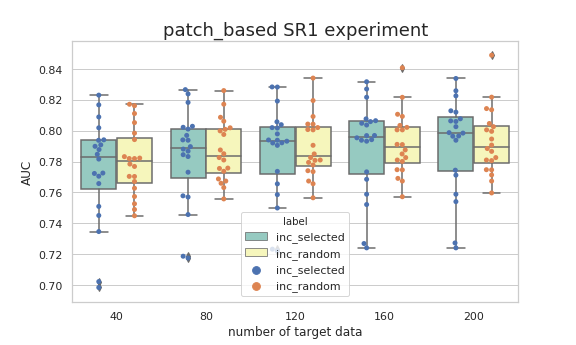
\includegraphics[width=\textwidth]{fig/SR1_num_patch.png}
        \caption{\label{fig:parallel1} Patch-based AUC for S1R1 Experiment}
    \end{minipage}
    \hfil
\end{figure}
\begin{figure}[H]
    \hfil
    \begin{minipage}[t]{0.9\textwidth}
        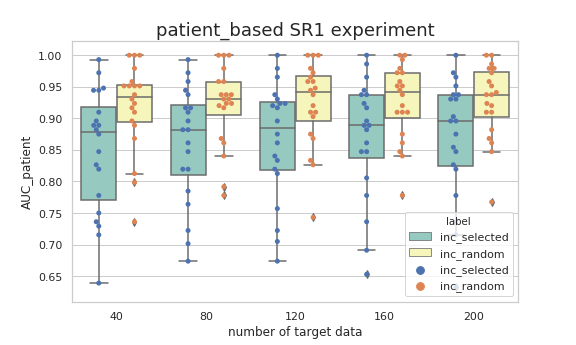
\includegraphics[width=\textwidth]{fig/SR1_num_patient.png}
        \caption{\label{fig:parallel1} Patient-based AUC for S1R1 Experiment}
    \end{minipage}
    \hfil
\end{figure}


\section{Comparison of Fine-Tuning Experiments and Incremental Learning Experiments}
I compared the AUC performance of source data model (B1), fine-tuning model (F1), and selected incremental learning model (S1). The selected incremental learning model can't provide obvious difference by selection method. Another problem is that the performance incremental learning stop early compared with fine-tuning. I drew the validation loss diagram and found that the loss almost didn't decrease after first 50 epochs. This algorithm may estimate too much on the first few data it selected and only find a local minimum in training process.

\begin{figure}[H]
    \hfil
    \begin{minipage}[t]{0.9\textwidth}
        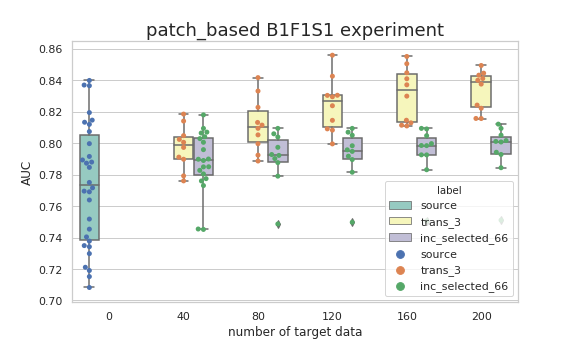
\includegraphics[width=\textwidth]{fig/B1F1S1_num_patch.png}
        \caption{\label{fig:parallel1}Patch-based AUC for B1F1S1 Experiment}
    \end{minipage}
    \hfil
\end{figure}
\begin{figure}[H]
    \hfil
    \begin{minipage}[t]{0.9\textwidth}
        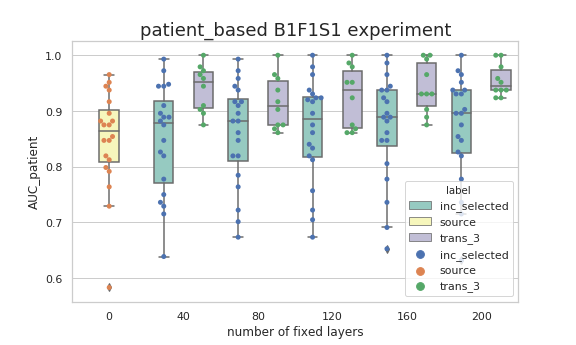
\includegraphics[width=\textwidth]{fig/B1F1S1_num_patient.png}
        \caption{\label{fig:parallel1}Patient-based AUC for B1F1S1 Experiment}
    \end{minipage}
    \hfil
\end{figure}
\begin{figure}[H]
    \hfil
    \begin{minipage}[t]{0.9\textwidth}
        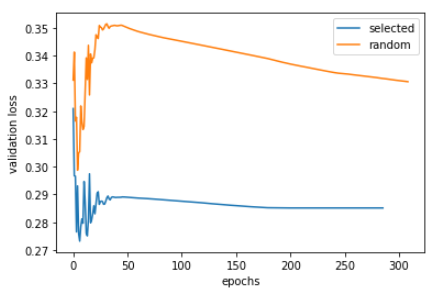
\includegraphics[width=\textwidth]{fig/loss.png}
        \caption{\label{fig:parallel1} Validation Loss of Selected/Random Incremental Learning}
    \end{minipage}
    \hfil
\end{figure}